\documentclass[12pt]{article}

\usepackage[T1]{fontenc}
\usepackage[a4paper, left=3cm, right=2cm, top=3cm, bottom=2cm]{geometry}
\usepackage[dvipsnames]{xcolor}
\usepackage[toc]{glossaries}
\usepackage{authblk}
\usepackage{cite}
\usepackage{fontspec}
\usepackage{graphicx}
\usepackage{hyperref}
\usepackage{relsize}
\usepackage{setspace}
\usepackage{subcaption}
\usepackage{verbatimbox}
\usepackage{listings}
\usepackage[english, portuguese]{babel}
    \addto\captionsportuguese{\renewcommand*\bibname{Referências}}
    \addto\captionsportuguese{\renewcommand*\contentsname{Sumário}}

\newcommand\myshade{85}
\newcommand{\pprime}{\ensuremath{^{\prime}}}
\newcommand{\RNum}[1]{\uppercase\expandafter{\romannumeral #1\relax}}
\renewcommand\Authsep{, }
\renewcommand\Authand{, }
\renewcommand\Authands{ e }
\providecommand{\keywords}[1]{%
  \small
  \textbf{\textit{\iflanguage{english}{Keywords}{Palavras-chave} ---}} #1%
}

\hypersetup{
  pdftitle   = {Relatório do Trabalho Prático, INE5645 — Trabalho II: Programação Distribuída},
    pdfauthor  = {Pedro Santi Binotto, Gabriel Lemos da Silva, Bruno Alexandre Schmitt Costa},
    pdfsubject = {Resumo em Português},
    linkcolor  = black,
    citecolor  = black,
    urlcolor   = black,
    colorlinks = true,
    filecolor  = black,
    linktoc    = page
}%

\lstset{
  basicstyle=\small\ttfamily,
  columns=flexible,
  breaklines=true
}

\graphicspath{ {./resources/} }

% \newglossaryentry{gls} {
%   name={GLS},
%   description={Glossary entry}
% }

\title{Relatório do Trabalho Prático \\ [0.2em]\smaller{}INE5645 -- Trabalho \RNum{2}: Programação Distribuída}
\author[1]{Pedro Santi Binotto [20200634]\thanks{\texttt{pedro.binotto@grad.ufsc.br}}}
\author[1]{Gabriel Lemos da Silva [18200628]\thanks{\texttt{glemoss.dev@gmail.com}}}
\author[1]{Bruno Alexandre Schmitt Costa [17105532]\thanks{\texttt{bruno\_alexandre.s@hotmail.com}}}
\date{\today}
\affil[1]{Departamento de Informática e Estatística, Universidade Federal de Santa Catarina}

\makeglossaries

\begin{document}
\begin{titlepage}
\selectlanguage{portuguese} 
\maketitle
\thispagestyle{empty}

\begin{abstract}
  Este documento busca registrar os detalhes da implementação técnica e casos de teste referentes ao trabalho proposto em \href{https://github.com/PedroBinotto/INE5645-2025.01/blob/84814a13247d42dd6bec83c8b5ae65c7805c7bfb/trabalho_2/project/INE5645_trabalho2.pdf}{"Trabalho
  2: Programação Distribuída"}.


\end{abstract}

\end{titlepage}

\tableofcontents

\printglossary[title=Glossário, toctitle=Glossário]

\section{Introdução}

\paragraph{}
Este relatório apresenta o desenvolvimento do protótipo de um modelo de memória compartilhada distribuída entre
múltiplas instâncias de um programa (processos). 

\subsection{Proposta}
\paragraph{}
Conforme especificado no enunciado do projeto, o objetivo central é criar uma abstração inter--processos onde um espaço
de endereçamento de memória é logicamente unificado e acessível por múltiplos processos, embora seus blocos
constituintes estejam fisicamente distribuídos entre eles (podendo ser em uma mesma máquina física ou não). Além disso,
um requisito central da proposta é também a implementação de um mecanismo de \textit{caching} local a cada processo, de
forma que seja mantida a coerência de \textit{caches} no nível da rede de processos:

\begin{quote}
  Operações tanto de leitura quanto de escrita podem acessar blocos locais ou remotos, ou, ainda, locais e remotos. Para acessos remotos, o processo solicitante deve fazer uma cópia do(s) bloco(s) de interesse e mantê-la em uma cache local. Dessa forma, leituras sobre o bloco podem ser feitas pela cache, caso haja uma cópia do bloco de interesse disponível.
  No caso de leituras e leituras sucessivas, se o processo tiver uma cópia válida do bloco, basta ler da sua cache. No
  caso de escritas, o processo deve atualizar o valor do bloco no conteúdo do dono do bloco e gerar uma invalidação das
  cópias daquele bloco em caches de outro processos. Este procedimento é comum na implementação de mecanismos para
  coerência de cache e chama-se \textit{invalidação na escrita}.
\end{quote}

\section{Solução}
\paragraph{}
Para a elaboração da implementação do projeto, foram adotadas as seguintes ferramentas e tecnologias:

\begin{description}
  \item[C++:] A linguagem de programação escolhida para a elaboração do projeto foi o C++, como apresenta algumas
    facilidades a mais quando comparado com a especificação pura do C (orientação a objetos, etc...) mas mantém a
    granularidade de controle, da qual nos aproveitamos para modelar a alocação de memória, além de ser facilmente
    integrado com o sistema de comunicação MPI;
  \item[OpenMPI:] O OpenMPI é uma das mais populares e difundidas implementações da especificação MPI, sendo facilmente
    instalado na maioria dos sistemas operacionais UNIX-like.
\end{description}

\paragraph{}
Durante o desenvolvimento, foi realizada pesquisa principalmente nos recursos \cite{mpitutorial}, \cite{openmpi} e
\cite{cppreference}.


\subsection{Arquitetura}
\paragraph{}
A arquitetura do protótipo adota um modelo SIMD (Single Instruction, Multiple Data), onde cada processo MPI executa o
mesmo código, mas assume papéis distintos com base em seu rank. O sistema é construído sobre a API MPI, utilizando um
modelo de passagem de mensagens e \textit{threads} para gerenciar a comunicação e a coerência de cache.

\subsubsection{Visão Geral}
\paragraph{}
O projeto implementa dois tipos distintos de processo para realizar as soluções de comunicação e compartilhamento de
memória:

\begin{description}
  \item[\textit{Worker Processes}:] São os processos de \textit{rank} \(0 .. N\) (em que \(N\) é o parâmetro de \texttt{N\_PROCS} informado pelo usuário), que tem o papel de gerenciar blocos de memória:
    \begin{itemize}
      \item Mantém localmente os blocos de memória que foram atribuídos à instância;
      \item Mantém um índice de todos os \textit{maintainers} para os blocos que estão alocados remotamente -- ou seja,
        em outras instâncias -- de forma que pode consultar estes blocos através de uma mensagem MPI ao bloco
        responsável;
      \item Mantém uma \textit{cache} local dos blocos remotos que já foram acessados, invalidando-a quando recebe uma
        notificação de atualização de bloco (via \textit{broadcast});
      \item Realiza o controle de leitura e escrita sobre os blocos locais, prevenindo condições de corrida e
        notificando o \textit{broadcaster} quando ocorre uma atualização a um dos blocos locais;
    \end{itemize}
  \item[\textit{Broadcaster Process}:] É o processo identificado pelo \textit{rank} \(N + 1\), e desempenha o papel de repassar as mensagens de notificação em \textit{broadcast} para todos os processos \textit{worker}:
    \begin{itemize}
      \item Não tem conhecimento do estado da aplicação (blocos alocados), apenas recebe as mensagens de notificação dos
        processos \textit{worker} (contendo o ID do bloco atualizado e o \textit{timestamp} da operação) e realiza o
        \textit{broadcast} para os demais processos;
    \end{itemize}
\end{description}

\paragraph{}
A determinação da relação de \textit{maintainers} para os blocos alocados é dada no \textit{startup} da aplicação,
produzindo um mapa estático que perdurará até o fim da execução. O tamanho e número de blocos, assim como o número de
\textit{workers} é, da mesma forma, imutável, sendo informado ao processo através dos parâmetros da linha de comando.

\paragraph{}
A organização pode ser visualizada através das seguintes representações gráficas:

\begin{figure}[h!]
\centerline{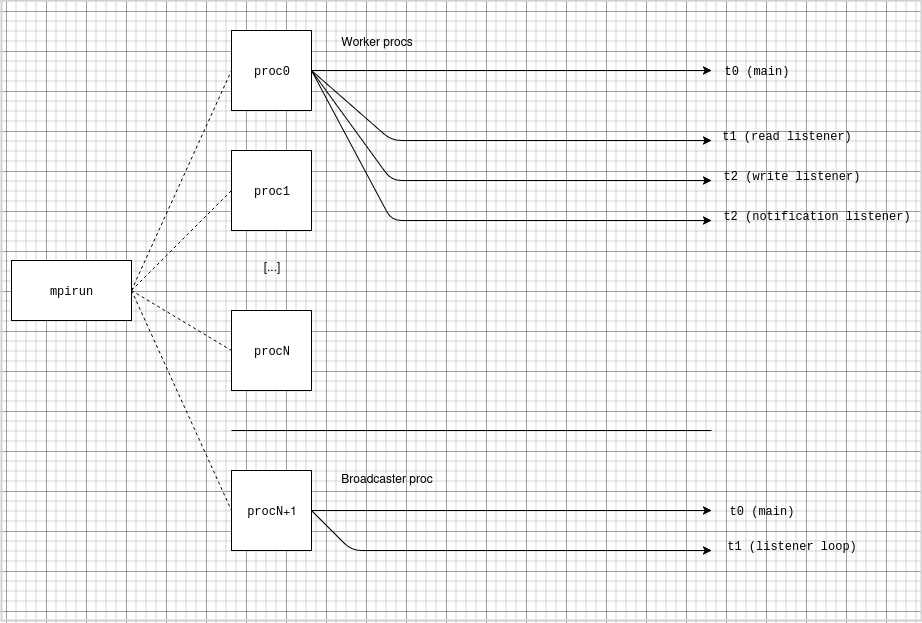
\includegraphics[totalheight=6cm]{INE5645-slide-2.drawio.png}}
  \caption{Visão geral da organização dos processos}
  \label{fig:topologia}
\end{figure}

\begin{figure}[h!]
\centerline{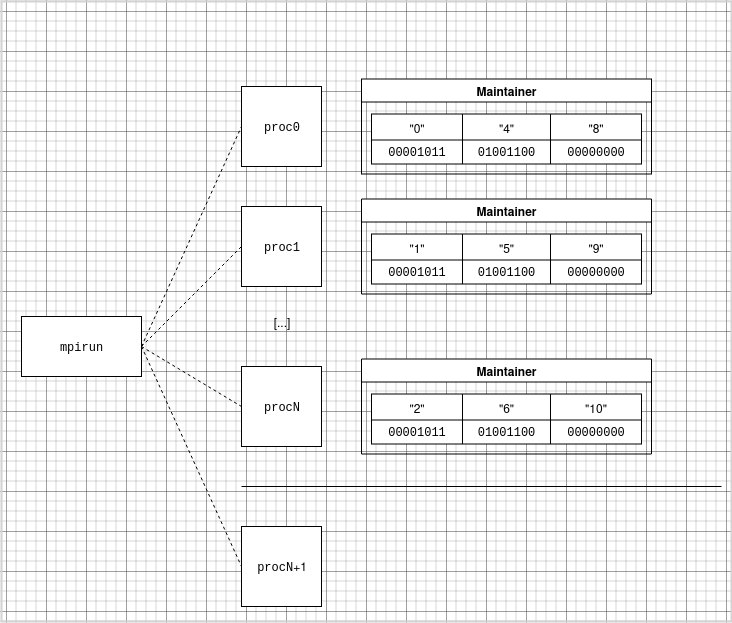
\includegraphics[totalheight=6cm]{INE5645-slide-3.drawio.png}}
  \caption{Representação da alocação de blocos}
  \label{fig:allocation}
\end{figure}

\begin{figure}[h!]
\centerline{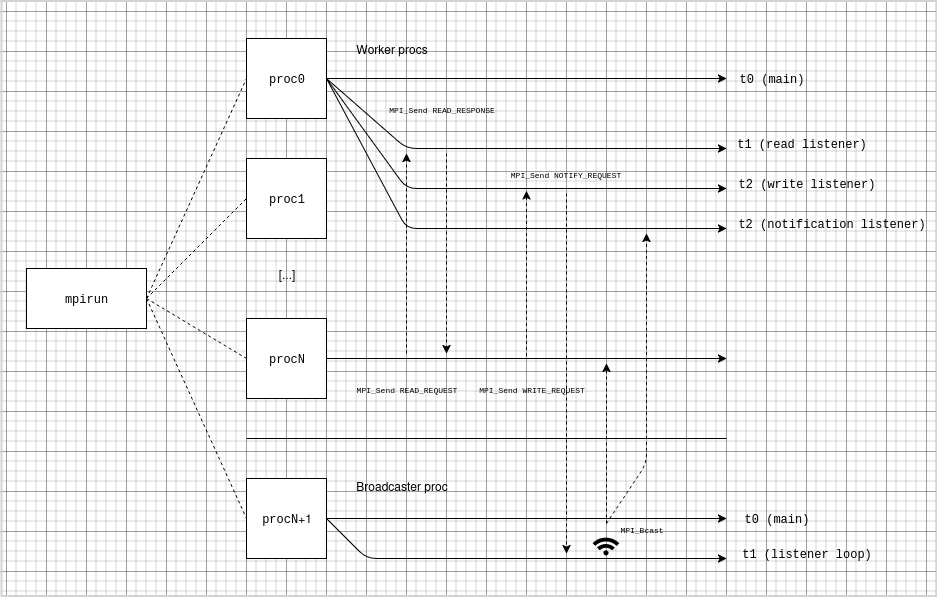
\includegraphics[totalheight=6cm]{INE5645-slide-6.drawio.png}}
  \caption{Representação do ciclo de vida dos processos}
  \label{fig:lifecycle}
\end{figure}

\subsection{Implementação}
\subsubsection{Acesso aos dados}
\paragraph{}
A implementação interna dos processos descritos até então é realizada através de uma série de componentes e interfaces
de forma que, da perspectiva da \textit{thread} principal do processo \textit{worker}, a única API disponível oferece as
operações de \texttt{read} e \texttt{write} da classe de acesso de dados (no caso concreto, através de um
\textit{wrapper} desenvolvido para adequar-se à especificação de \texttt{le} e \texttt{escreve}, descrito na proposta do
trabalho), de forma que não é necessário "preocupar-se" com a diferença entre um acesso local e remoto, invalidação de
\textit{cache} e demais detalhes que são abstraídos pela classe de repositório e automatizado pelas \textit{threads}
auxiliares.

\begin{lstlisting}[
  language=C++,
  frame=single
  label=maincpp,
  caption={(\texttt{main.cpp}) A classe \texttt{UnifiedRepositoryFacade} oferece simples acesso de leitura e escrita à memória compartilhada, implementando os detalhes da lógica de acesso através do MPI e dos blocos locais:}
]
int escreve(int posicao, std::shared_ptr<uint8_t[]> buffer, int tamanho) {
  int num_blocks = registry_get(GlobalRegistryIndex::NumBlocks);
  int block_size = registry_get(GlobalRegistryIndex::BlockSize);
  int scoped_blocks = std::ceil(static_cast<double>(tamanho) / block_size);
  int final_pos = posicao + scoped_blocks;

  if (final_pos > num_blocks)
    return 1;

  for (int i = 0; i < scoped_blocks; i++) {
    block new_buf = std::make_shared<uint8_t[]>(block_size);
    std::memcpy(new_buf.get(), buffer.get() + (i * block_size), block_size);
    repository->write(posicao + i, new_buf);
    thread_safe_log_with_id(std::format(
        "Performing WRITE operation to block {0} at `main` level", posicao));
  }

  return 0;
}

int le(int posicao, std::shared_ptr<uint8_t[]> buffer, int tamanho) {
  int num_blocks = registry_get(GlobalRegistryIndex::NumBlocks);
  int block_size = registry_get(GlobalRegistryIndex::BlockSize);
  int scoped_blocks = std::ceil(static_cast<double>(tamanho) / block_size);
  int final_pos = posicao + scoped_blocks;

  if (final_pos > num_blocks)
    return 1;

  for (int i = 0; i < scoped_blocks; i++) {
    block result = repository->read(posicao + i);
    std::memcpy(buffer.get() + (i * block_size), result.get(), block_size);
    thread_safe_log_with_id(std::format(
        "Performing READ operation to block {0} at `main` level", posicao));
  }

  return 0;
}
\end{lstlisting}

\paragraph{}
Isso é possível por que a classe utilizada pelo \textit{worker} (\texttt{UnifiedRepositoryFacade}) implementa um
\textit{proxy} para as classes especializadas \texttt{LocalRepository} (mantém os registros locais e realiza o
gerenciamento de acessos simultâneos) e \texttt{RemoteRepository} (oferece acesso remoto aos demais processos e mantém
\textit{caches} locais para operações repetidas):

\begin{figure}[h!]
\centerline{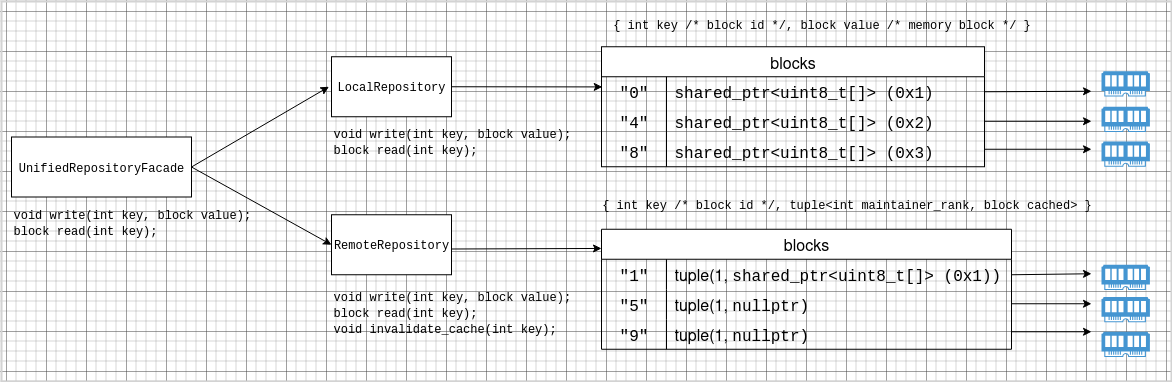
\includegraphics[totalheight=6cm]{INE5645-slide-5.drawio.png}}
  \caption{Implementação dos \textit{repositories} (\texttt{lib.hpp})}
  \label{fig:repositories}
\end{figure}

\paragraph{}
Assim, a \textit{thread} \texttt{main} realiza as operações através desta interface, enquanto as \textit{threads}
\texttt{read} e \texttt{write} recebem e processam requisições dos outros processos (para \textit{leitura} e
\textit{escrita} nos blocos mantidos, respectivamente) e a \textit{thread} \texttt{notification} escuta por eventos de
atualização, que serão recebidos via \textit{broadcast} do processo \textit{broadcaster}. Ao receber um evento de
notificação, uma chamada é realizada à instância de \texttt{RemoteRepository::invalidate\_cache} para que o registro
local (\textit{cached}) seja \textit{invalidado} (\verb|shared_ptr<uint_8[]>| (\textit{bytearray}) \(\Rightarrow\) \texttt{nullptr}
(NULL)).

\subsubsection{Comunicação e codificação de mensagens}
\paragraph{}
A comunicação entre processos é dividida em dois tipos principais (\texttt{lib.hpp}, \texttt{servers.hpp}, \texttt{servers.cpp}):

\begin{description}
  \item[Comunicação Individual (\textit{point--to--point}):] Engloba as mensagens enviadas entre um processo e outro
    através do MPI (via \texttt{MPI\_Send} e \texttt{MPI\_Recv}). Na implementação do sistema, este tipo de comunicação
    foi empregado nos seguintes cenários:
    \begin{description}
      \item[Operações de leitura:] As operações de \textit{leitura} remota (de um processo para o bloco mantido por
        outro) são realizadas através de dois pares send/receive: o processo solicitante envia uma requisição
        (\texttt{MPI\_Send} com a \textit{tag} \texttt{MESSAGE\_TAG\_BLOCK\_READ\_REQUEST} e o ID do bloco desejado) que
        será interpretada pela \textit{thread} \texttt{read} do processo remoto, e recebe o
        \textit{receive} de confirmação. Após isso, o processo \textit{maintainer} do bloco solicitado realiza um
        \texttt{MPI\_Send} com a \textit{tag} \texttt{MESSAGE\_TAG\_BLOCK\_READ\_RESPONSE} e o conteúdo do bloco solicitado;
      \item[Operações de escrita:] As operações de \textit{escrita} remota (de um processo para o bloco mantido por
        outro) são realizadas através de dois pares send/receive: o processo solicitante envia uma requisição
        (\texttt{MPI\_Send} com a \textit{tag} \texttt{MESSAGE\_TAG\_BLOCK\_WRITE\_REQUEST} e o ID e \textit{bytes} para
        escrever no bloco desejado) que será interpretada pela \textit{thread} \texttt{read} do processo remoto, e recebe
        o \textit{receive} de confirmação. Após isso, o processo \textit{maintainer} do bloco solicitado realiza um a 
        escrita dos dados e solicita uma notificação de atualização ao processo \textit{broadcaster};
      \item[Solicitação de notificação:] Quando o processo \textit{maintainer} realiza a escrita a um bloco, este
        realiza uma chamada de \texttt{MPI\_Send} ao processo \textit{broadcaster} com a \textit{tag}
        \texttt{MESSAGE\_TAG\_BLOCK\_UPDATE\_NOTIFICATION} e o ID do bloco, acompanhado de um \textit{timestamp} UNIX
        indicativo do momento da escrita do bloco;
    \end{description}
  \item[Comunicação Coletiva:] Engloba as mensagens enviadas entre vários processos de uma só vez. Na implementação do
    sistema, a única primitiva de comunicação coletiva do MPI empregada foi o \texttt{MPI\_Bcast}, que representa uma
    comunicação de \textit{um--para--muitos} de uma mesma mensagem. Esta primitiva foi utilizada no seguinte cenário:
    \begin{description}
      \item[Transmissão de notificação:] Quando o processo \textit{broadcaster} recebe uma requisição de notificação de
        um processo \textit{worker} (ocorre logo em seguida de uma operação de escrita bem-sucedida), este se encarrega
        de repassar para todos os \textit{workers} que o bloco informado foi atualizado, para que estes possam invalidar
        suas \textit{caches}. Isto é implementado através de uma chamada à \texttt{MPI\_Bcast}, repassando a mensagem
        (composta do ID e \textit{timestamp} da escrita) em um \textit{broadcast} que será recebido pela \textit{thread}
        \texttt{notification} de cada processo (e ignorado pelo processo que enviou a requisição, por motivos óbvios).
    \end{description}
\end{description}

\section{Casos de teste e verificação}
\subsection{Coerência de cache}
\paragraph{}
O mecanismo de coerência de \textit{cache} e prevenção de acesso inválido (\textit{race--condition}) pode ser verificado
ao realizar uma análise cronológica das operações registradas nos arquivos de \textit{log} e comparar os estados em
diferentes processos no mesmo ponto no tempo (identificável pela \textit{timestamp} no prefixo de cada linha do log).
Assim, é possível realizar cruzamento dos dados ao concatenar (via \texttt{cat}) os arquivos de \textit{log} e aplicar
uma ordenação pelo \textit{timestamp}, produzindo um documento que representa a ordem dos acontecimentos registrados por
diferentes processos conforme a execução do código progride.

\begin{lstlisting}[
  frame=single
  label=log,
  caption={Neste trecho de \textit{log} é possível observar a ordem com que os eventos ocorrem entre os diferentes
  processos em execução (no exemplo, uma requisição de \textit{escrita} para o bloco \texttt{2} é enviada do processo
  \texttt{0} para o processo \texttt{2}, que realiza a operação e solicita a transmissão da notificação ao processo
  \texttt{4 (broadcaster)}):}
]
[1752262034] (@proc 0) Performing WRITE operation to block 2 at `main` level
[1752262034] (@proc 0) Read listener probing...
[1752262034] (@proc 0) Read thread started
[1752262034] (@proc 0) Received method call to execute remote WRITE operation to block 2 with value 01100111 11000110 01101001 01110011 01010001 11111111 01001010 00000000  on process ID 2
[1752262034] (@proc 0) Sending WRITE request of key: 2, value: 01100111 11000110 01101001 01110011 01010001 11111111 01001010 00000000  serialized as 00000010 00000000 00000000 00000000 01100111 11000110 01101001 01110011 01010001 11111111 01001010 00000000  over MPI
[1752262034] (@proc 0) Started as worker process
[1752262034] (@proc 0) Started helper threads
[1752262034] (@proc 0) WRITE operation to block 2 called at remote repository level
...
[1752262035] (@proc 2) Allocated memory for buffer
[1752262035] (@proc 2) Cached data not available for block 0. Performing remote access request...
[1752262035] (@proc 2) Completed READ request from process of ID 1 successfully. Sending out response for block 2...
[1752262035] (@proc 2) Completed WRITE request from process of ID {0} successfully.
[1752262035] (@proc 2) Constructed object: key 2, value 01100111 11000110 01101001 01110011 01010001 11111111 01001010 00000000  from raw message buffer 00000010 00000000 00000000 00000000 01100111 11000110 01101001 01110011 01010001 11111111 01001010 00000000 
[1752262035] (@proc 2) Copied buffer to memory
[1752262035] (@proc 2) DEBUG: Current local allocated block configuration: 
[1752262035] (@proc 2) Decoding write message from bytearray buffer: 00000010 00000000 00000000 00000000 01100111 11000110 01101001 01110011 01010001 11111111 01001010 00000000 
[1752262035] (@proc 2) Detected READ operation request at `listener` level
[1752262035] (@proc 2) Detected WRITE operation request at `listener` level
[1752262035] (@proc 2) Encoding notification message from of key: 2, timestamp: 1752262035 as bytearray buffer 00000010 00000000 00000000 00000000 10010011 01100101 01110001 01101000 00000000 00000000 00000000 00000000 
[1752262035] (@proc 2) Processing READ operation request at `handler` level...
[1752262035] (@proc 2) Processing WRITE operation request at `handler` level...
[1752262035] (@proc 2) READ operation to block 0 called at remote repository level
[1752262035] (@proc 2) READ operation to block 2 called at local repository level
[1752262035] (@proc 2) Read listener probing...
[1752262035] (@proc 2) Sending out update notification request for block 2...
\end{lstlisting}

\subsection{Cenários de teste e casos críticos}
\paragraph{}

\newpage
\section{Bibliografia}
\bibliographystyle{plain}
\bibliography{references}

\end{document}

